%% Code, logged results and the scripts that generate every number and table in this paper:
%% https://github.com/ibrahimghauri009/capri-federated-unlearning-ids
\documentclass[pdflatex,sn-mathphys-num,iicol]{sn-jnl}

\usepackage{graphicx}%
\usepackage{multirow}%
\usepackage{amsmath,amssymb,amsfonts}%
\usepackage{amsthm}%
\usepackage{mathrsfs}%
\usepackage[title]{appendix}%
\usepackage{xcolor}%
\usepackage{textcomp}%
\usepackage{manyfoot}%
\usepackage{booktabs}%
\usepackage{array}%
\usepackage{placeins}%
\usepackage{algorithm}%
\usepackage{algorithmicx}%
\usepackage{algpseudocode}%
\usepackage{tikz}%
\usetikzlibrary{arrows.meta,positioning,fit,calc,backgrounds}%

\newcommand{\Efit}{E_{\mathrm{fit}}}
\newcommand{\Echk}{E_{\mathrm{chk}}}
\newcommand{\DD}{\mathrm{DD}_{\rho}}
\newcommand{\DDdef}{\mathrm{DDdef}_{\rho}}
\newcommand{\rprobe}{r^{\mathrm{probe}}_c}
\definecolor{capri}{RGB}{214,230,245}
\definecolor{capriline}{RGB}{31,94,160}

\hypersetup{pdftitle={Sole-Holder Deletion in Federated Intrusion Detection: Measuring, Predicting and Repairing Lost Attack-Family Detection},
  pdfauthor={Ibrahim Ghauri, Okasha Yamin},
  pdfkeywords={Federated unlearning, Intrusion detection, Machine unlearning, Non-IID federated learning, Internet of Things security, Right to erasure}}

\makeatletter\@ifpackageloaded{natbib}{\setlength{\bibsep}{1pt plus 0.3ex}}{}\makeatother
\raggedbottom

\begin{document}

\title[Sole-holder deletion in federated intrusion detection]{Sole-Holder Deletion in Federated Intrusion Detection: Measuring, Predicting and Repairing Lost Attack-Family Detection}

\author*[1]{\fnm{Ibrahim} \sur{Ghauri}}\email{i232653@isb.nu.edu.pk}
\equalcont{These authors contributed equally to this work.}
\author[1]{\fnm{Okasha} \sur{Yamin}}\email{i232525@isb.nu.edu.pk}
\equalcont{These authors contributed equally to this work.}
\affil[1]{\orgdiv{Department of Data Science}, \orgname{National University of Computer and Emerging Sciences (FAST-NUCES)}, \orgaddress{\city{Islamabad}, \country{Pakistan}}}

\abstract{Federated learning lets organisations train a shared intrusion detection system without pooling traffic, and federated unlearning removes a departing organisation's contribution. Unlearning is judged by closeness to a model retrained without the departing client, a criterion that fails when that client is the only holder of an attack family: correct unlearning then removes the detector's ability to recognise the family, and aggregate metrics hide it. This study measures this capability loss and proposes CAPRI (capability-preserving, risk-informed federated unlearning): CAPRI-Audit estimates per-family risk before deletion from server-side information, and CAPRI-Guard, a plug-in repair, restores per-family recall from a small independently held exemplar set, judged against a lawful oracle that retrains with the same exemplars. On Edge-IIoTset and CICIoT2023 (<<len(DS['edge']['p1'])+len(DS['cic']['p1'])>> federated trainings, ten clients, six ownership scenarios, eight baselines), retraining removed <<pct(h1p('B1','mean_loss_S3'),1)>> of a learned family's recall when its sole holder left (FedEraser <<pct(h1p('B5','mean_loss_S3'),1)>>, gradient ascent <<pct(h1p('B4','mean_loss_S3'),1)>>), against less than <<pct(max(abs(h1p(mm,'mean_loss_S1')) for mm in ['B1','B4','B5'])+0.0005,1)>> under shared ownership (Holm-corrected $p=$ <<fp(h1p('B1','p_holm'))>>). CAPRI-Guard raised mean target-family recall after FedEraser from <<f(tgt('S3','B5','edge'))>> to <<f(tgt('S3','Guard[B5]','edge'))>> on Edge-IIoTset and reduced the detection-debt deficit by <<f(-rel(v('S3','Guard[B5]','dd_deficit','edge'),v('S3','B5','dd_deficit','edge')),0)>>\%, with membership inference at chance level. Plain fine-tuning on the same exemplars performed equally well, and on CICIoT2023 the repair raised benign false alarms to <<pct(v('S3','Guard[B1]','benign_far','cic'),0)>>. The audit outperformed a counts-based rule on families other clients still hold on Edge-IIoTset (F1 <<f(audit('m_c > 0 (non-trivial)','CAPRI-Audit (all signals)','f1','edge'),2)>> versus <<f(audit('m_c > 0 (non-trivial)','Rule-only (counts)','f1','edge'),2)>>) but not within CICIoT2023. Per-family evaluation is required to expose sole-holder loss, and lawful exemplars, rather than a specific repair mechanism, restore the lost capability.}

\keywords{Federated unlearning, Intrusion detection, Machine unlearning, Non-IID federated learning, Internet of Things security, Right to erasure}

\maketitle

%% ============================================================== 1
\section{Introduction}\label{sec:intro}

Federated learning (FL)~\cite{mcmahan2017} lets operators of Internet of Things (IoT) and industrial networks train a shared intrusion detection system (IDS) while each keeps its traffic local, which is attractive because each operator observes only part of the attack landscape~\cite{bilal2026,peng2025fdids,chunduru2025}. Federations are not static: an operator may leave, withdraw consent or exercise a legal right to erasure~\cite{gdpr2016}. Federated unlearning removes the departing client's contribution from the global model without retraining from scratch~\cite{cao2015,bourtoule2021,liu2021federaser,halimi2022,wu2022distill}.

Unlearning methods are almost universally evaluated by their closeness to the \emph{retrain oracle}, a model trained from the start without the departing client~\cite{liu2021federaser,halimi2022,liu2025starfish,yang2026arfu}. For an IDS this criterion has a blind spot. Attack families are unevenly distributed across organisations, and some are observed by a single member; when that member leaves, the retrain oracle has never seen the family, so a method that matches it perfectly also stops detecting it. Accuracy barely changes and the missed attacks are mostly classified as benign: correct unlearning can create a silent detection gap.

This effect is not measured in the literature reviewed here. Federated unlearning methods are mostly evaluated on images~\cite{kwon2026,patra2026,wang2025fedbt,liu2025starfish,zhang2025cgkd}; the two studies on intrusion detection report a pooled rare-category recall and treat closeness to retraining as success~\cite{yang2026arfu,wang2026fuids}; and federated IDS studies examine missing classes but never remove a client~\cite{bilal2026,chunduru2025,peng2025fdids}. No reviewed evaluation removes the sole holder of an attack family and reports detection per family.

This study asks: (RQ1) how much per-family detection is lost when the departing client is the sole holder of a family rather than one of several; (RQ2) whether this loss can be predicted before the deletion is approved, from information the server legitimately holds; and (RQ3) whether per-family recall can be restored above a floor without weakening the forgetting of the departing client. The contributions are:
\begin{itemize}
\item A controlled measurement of per-family capability loss under six ownership scenarios on two IoT intrusion datasets with eight baselines, showing that sole-holder deletion removes a learned family under exact retraining as well as approximate unlearning (Section~\ref{sec:res-rq1}).
\item The \emph{lawful oracle}, which retrains without the departing client but with an independently held exemplar set, so that restoring a family from lawful data is not counted as a failure to forget (Section~\ref{sec:method}).
\item CAPRI-Audit, a pre-deletion estimate of each family's recall from ownership counts, a leave-one-client-out estimate computed from the stored update history, and embedding separability (Section~\ref{sec:audit}).
\item CAPRI-Guard, a plug-in repair that keeps flagged families above a recall floor by dual ascent, evaluated against fine-tuning on the same exemplars, which shows that the exemplars, not the mechanism, account for the gain (Sections~\ref{sec:guard} and~\ref{sec:ablation}).
\item A leakage-controlled benchmark protocol and open implementation that regenerates every reported number from logged outputs.
\end{itemize}

Sections~\ref{sec:related}--\ref{sec:conclusion} present related work, the method, the setup, the results, the comparison with the base methods, the ablations, the discussion and the conclusion.

%% ============================================================== 2
\section{Related work}\label{sec:related}

\paragraph{Federated unlearning methods.} \emph{History-based} methods store per-round client updates and reconstruct the model without the departing client: FedEraser calibrates the stored updates with local epochs of the remaining clients and reports an expected $4\times$ speed-up over retraining~\cite{liu2021federaser}, and Starfish certifies closeness to retraining with a secret-shared history~\cite{liu2025starfish}. \emph{Gradient-ascent} methods let the departing client reverse its training: Halimi et al.\ use projected gradient ascent followed by a few federated rounds~\cite{halimi2022}, and Kwon et al.\ separate gradient ascent from a distillation-based preservation phase~\cite{kwon2026}. \emph{Distillation-based} methods subtract the client's historical updates and restore utility by knowledge distillation (KD) from the original model~\cite{wu2022distill}, use an uninformative teacher~\cite{wang2025fedbt} or recover the model from a small server dataset~\cite{zhang2025cgkd}; class-level variants use lightweight auxiliary heads~\cite{patra2026}. These methods are evaluated mostly on image data, against closeness to retraining.

\paragraph{Unlearning in intrusion detection.} ARFU-IDS~\cite{yang2026arfu} and FU-IDS~\cite{wang2026fuids} are, among the studies reviewed, the only federated unlearning methods evaluated on native tabular intrusion data. Both aim to preserve rare-attack detection, using attention-head or neuron-level attribution, and both report a single pooled rare-category recall on UNSW-NB15 together with closeness to retraining. MT-KD~\cite{shen2026mtkd} unlearns attack classes in a centralised IIoT IDS through multi-teacher distillation on traffic converted to images. None of these studies constructs exclusive ownership of an attack family, so the case in which the retraining reference itself loses a family does not arise.

\paragraph{Federated intrusion detection under label skew.} Bilal et al.~\cite{bilal2026} evaluate federated IDSs across Edge-IIoTset, CICIoT2023 and TII-SSRC-23 and show large losses under dataset shift; Chunduru Sri Abhijit et al.~\cite{chunduru2025} show that a class absent from clients is missed entirely by plain FedAvg; FD-IDS~\cite{peng2025fdids} uses distillation to cope with non-IID IoT data. At the model level, restricted softmax (FedRS)~\cite{li2021fedrs} limits the updates of classes a client does not hold, which is the mechanism that allows a sole-held family to be learned in the first place (Section~\ref{sec:setup}). None of these studies considers the removal of a client.

\paragraph{Privacy of unlearning.} A membership-inference attack (MIA)~\cite{shokri2017,yeom2018} tests whether a client's records are still remembered. Unlearning is itself an attack surface: malicious deletion requests can degrade a model~\cite{chen2025fedmua}, and the difference between the models before and after unlearning can leak information about the forgotten data~\cite{zhou2026fuia}, an idea Section~\ref{sec:res-ext} applies to attack families.

Table~\ref{tab:related} summarises the key studies. The present study differs in three respects: it constructs sole-holder deletions on native IDS data, it evaluates every attack family separately, and it judges forgetting against a lawful oracle rather than against plain retraining.

\begin{table*}[t]
\caption{Summary of key related studies. PF: detection reported per attack family after unlearning; SH: the departing client is the only holder of a class or family; FU: federated unlearning.}\label{tab:related}
\scriptsize
\setlength{\tabcolsep}{3pt}
\begin{tabular*}{\textwidth}{@{\extracolsep\fill}>{\raggedright\arraybackslash}p{2.9cm}>{\raggedright\arraybackslash}p{3.5cm}>{\raggedright\arraybackslash}p{3.5cm}>{\raggedright\arraybackslash}p{3.5cm}cc@{}}
\toprule
Study (theme) & Data & Method & Success criterion & PF & SH \\
\midrule
FedEraser~\cite{liu2021federaser} (FU) & Adult, Purchase, MNIST, CIFAR-10 & Calibrated stored updates & Closeness to retraining & no & no \\
Halimi et al.~\cite{halimi2022} (FU) & MNIST, EMNIST, CIFAR-10 & Projected gradient ascent + FL rounds & Closeness to retraining & no & no \\
Wu et al.~\cite{wu2022distill} (FU) & MNIST, CIFAR-10, GTSRB & Update subtraction + distillation & Backdoor removal, accuracy & no & no \\
Starfish~\cite{liu2025starfish} (FU) & MNIST, Fashion-MNIST, CIFAR-10 & Secret-shared history, two-party computation & Certified closeness to retraining & no & no \\
Kwon et al.~\cite{kwon2026} (FU) & MNIST, CIFAR-10/100, Tiny-ImageNet & Gradient ascent + KD restoration & Forget drop, retained accuracy & no & no \\
FedDAM~\cite{patra2026} (class unlearning) & CIFAR-10/100, ImageNet-100 & Auxiliary head, dual momentum & Forget/retain accuracy & no & no \\
MT-KD~\cite{shen2026mtkd} (IDS, centralised) & CIC-IDS2017, USTC-TFC2016 & Multi-teacher distillation & Forget/retain accuracy & no & no \\
ARFU-IDS~\cite{yang2026arfu} (FU, IDS) & UNSW-NB15, CICIoT2023, IoTID20 & Attention-head attribution & Closeness to retraining, pooled rare recall & no & no \\
FU-IDS~\cite{wang2026fuids} (FU, IDS) & UNSW-NB15, CICIoT2023, IoTID20 & Neuron-level gradient scaling & Pooled rare recall, audit pass rate & no & no \\
Bilal et al.~\cite{bilal2026} (FL-IDS) & Edge-IIoTset, CICIoT2023, TII-SSRC-23 & FedAvg, FedProx, FedNova & Macro-F1, cross-dataset transfer & -- & -- \\
Chunduru et al.~\cite{chunduru2025} (FL-IDS) & CSE-CIC-IDS2018, UNSW-NB15, Edge-IIoTset & Personalised transfer learning & Per-class recall & -- & -- \\
\midrule
This study (FU, IDS) & Edge-IIoTset, CICIoT2023 & Audit + exemplar repair & Per-family recall vs.\ lawful oracle & yes & yes \\
\botrule
\end{tabular*}
\end{table*}

%% ============================================================== 3
\section{Proposed methodology}\label{sec:method}

\subsection{Problem formulation}\label{sec:problem}

A federation of $K$ clients trains a detector $f_\theta$ over $C+1$ classes (benign traffic and $C$ attack families) with FedAvg~\cite{mcmahan2017}. Client $k$ holds $n_{k,c}$ training records of class $c$. Training produces the global model $\theta_T$; the server stores the global model before every round $t$ and every client update $\Delta_{k,t}$ with its aggregation weight $w_{k,t}$. Client $u$ requests deletion. For each family $c$ the departing client's \emph{share} and the \emph{remaining support} are
\begin{equation}
s_c=\frac{n_{u,c}}{\sum_k n_{k,c}},\qquad m_c=\sum_{k\neq u} n_{k,c}.
\end{equation}
Let $r_c(\theta)$ denote the recall of family $c$ on the test set and $\mathcal{F}$ the set of evaluable families. For a recall floor $\rho$, the \emph{detection debt} and its continuous counterpart, the \emph{detection-debt deficit}, are
\begin{align}
\DD(\theta)&=\textstyle\sum_{c\in\mathcal{F}}\mathbf{1}[r_c(\theta)<\rho],\\
\DDdef(\theta)&=\textstyle\sum_{c\in\mathcal{F}}\max\bigl(0,\rho-r_c(\theta)\bigr).
\end{align}
An unlearning method $U$ maps $\theta_T$ and the history to an unlearned model $\theta_u$. The \emph{retrain oracle} $\theta^{\mathrm{RT}}$ is trained from the same initialisation without client $u$. A family is \emph{at risk} if $r_c(\theta_T)\ge\rho$ but $r_c(\theta^{\mathrm{RT}})<\rho$: its loss is caused by the deletion, independently of any approximation. If $m_c=0$, erasure lawfully removes the capability (a \emph{required} loss); if $m_c>0$, the loss is \emph{collateral}.

The server also holds an \emph{exemplar set} $E$ of $q$ records per class, obtained independently of every client (for example, public attack traces or a security team's curated library) and therefore not subject to the deletion request. It is split into a fitting part $\Efit$ and a check part $\Echk$. The \emph{lawful oracle} $\theta^{\mathrm{LO}}$ retrains without client $u$ but with $\Efit$ as an additional participant. Forgetting of a method that uses exemplars is judged against $\theta^{\mathrm{LO}}$, because restoring a family from lawfully held data is not a failure to forget the departing client.

\begin{figure*}[t]
\centering
\begin{tikzpicture}[
  font=\footnotesize, node distance=5mm and 5mm,
  box/.style={draw, rounded corners=2pt, align=left, inner sep=4pt, text width=#1},
  box/.default=3.4cm,
  prop/.style={box=#1, fill=capri, draw=capriline, thick},
  prop/.default=3.4cm,
  arr/.style={-{Stealth[length=2mm]}, thick},
  lbl/.style={font=\scriptsize\itshape}]
% middle column (proposed method)
\node[prop=5.8cm] (audit) {\textbf{CAPRI-Audit} (before the deletion is approved)\\[1pt]
 ownership: $s_c$, $\log(1+m_c)$ from label counts\\
 contribution: recall $\rprobe$ of leave-$u$-out estimate $\hat\theta_{-u}$ on $\Echk$\\
 separability: prototype margin of $\hat\theta_{-u}$\\
 binomial GLM $\rightarrow\hat r_c$ $\rightarrow$ Required / Collateral / Safe\\
 output: flagged set $A$ = Required $\cup$ Collateral};
\node[box=5.8cm, below=6mm of audit] (base) {\textbf{Base unlearning} $U$ (any method)\\ retrain (B1), gradient ascent (B4), FedEraser (B5) $\rightarrow\theta_u$};
\node[prop=5.8cm, below=6mm of base] (guard) {\textbf{CAPRI-Guard} (after unlearning)\\[1pt]
 $\min_\theta\ \mathrm{KL}(\theta_u\Vert\theta)+\gamma\Vert\theta-\theta_u\Vert^2+\sum_{c\in A}\lambda_c\,\mathrm{CE}_c$ on $\Efit$\\
 $\lambda_c\leftarrow\mathrm{clip}(\lambda_c+\eta(\rho-r_c),0,\lambda_{\max})$, $r_c$ on $\Echk$\\
 MIA check against the lawful oracle $\rightarrow\theta_G$};
% left column (inputs)
\node[box=3.1cm, left=9mm of audit.north west, anchor=north east] (fed) {\textbf{Federated training}\\ $K$ clients, FedAvg with restricted softmax; server stores $\theta_T$, updates $\Delta_{k,t}$, weights $w_{k,t}$, label counts $n_{k,c}$};
\node[box=3.1cm, below=5mm of fed] (req) {\textbf{Deletion request}\\ client $u$ leaves; its data must be forgotten};
\node[prop=3.1cm, left=9mm of guard.west, anchor=east] (ex) {\textbf{Lawful exemplars} $E$\\ $q$ records per class, held independently of all clients; $E=\Efit\cup\Echk$};
% right column (evaluation)
\node[box=3.3cm, right=15mm of audit.north east, anchor=north west] (eval) {\textbf{Evaluation}\\[1pt]
 capability: per-family recall, $\DD$, deficit, collateral loss, silent misses, benign false alarms\\[2pt]
 forgetting vs.\ lawful oracle: membership inference, forget-set accuracy, relearning\\[2pt]
 audit: precision, recall, F1};
\node[box=3.3cm, below=5mm of eval] (ref) {\textbf{References}\\ retrain oracle $\theta^{\mathrm{RT}}$ (defines at-risk families); lawful oracle $\theta^{\mathrm{LO}}$ = retrain $+\,\Efit$; control B8 = fine-tuning of $\theta_u$ on $\Efit$};
% arrows
\draw[arr] (fed) -- (req);
\draw[arr] (req.east) -- ++(4mm,0) |- ([yshift=4mm]audit.west);
\draw[arr] (ex.east) -- (guard.west);
\draw[arr, dashed] ([yshift=2mm]ex.east) -- ++(6mm,0) |- node[pos=0.3, sloped, below, lbl]{$\Echk$} ([yshift=-6mm]audit.west);
\draw[arr] (audit) -- node[right, lbl]{approve} (base);
\draw[arr] (base) -- node[right, lbl]{$\theta_u$} (guard);
\draw[arr] ([yshift=-4mm]audit.east) -- ++(4mm,0) |- node[pos=0.25, sloped, below, lbl]{flags $A$} ([yshift=4mm]guard.east);
\draw[arr] ([yshift=-4mm]guard.east) -- ++(10mm,0) |- node[pos=0.25, sloped, below, lbl]{repaired $\theta_G$} ([yshift=-4mm]eval.west);
\draw[arr, dashed] (ref.north) -- (eval.south);
\end{tikzpicture}
\caption{Architecture of CAPRI. Shaded components are proposed in this study; the federated training, base unlearning methods and evaluation references are held fixed for all methods. CAPRI-Audit runs before the deletion is approved and uses only information the server already holds; CAPRI-Guard repairs any base method's output from the lawful exemplar set and is judged against the lawful oracle.}\label{fig:arch}
\end{figure*}

\subsection{CAPRI-Audit}\label{sec:audit}

CAPRI-Audit (Fig.~\ref{fig:arch}) estimates, before the deletion is approved, the recall each family will have once client $u$ is removed. It uses three signals.

\emph{Ownership.} The share $s_c$ and $\log(1+m_c)$ from the per-client label counts, which FedAvg servers commonly receive for weighting.

\emph{Contribution.} A leave-$u$-out estimate $\hat\theta_{-u}$ is computed from the stored history without contacting any client: in every round, the aggregate of all updates is replaced by the aggregate of the remaining clients' updates with renormalised weights,
\begin{equation}\label{eq:loo}
\hat\theta_{-u}=\theta_T+\sum_{t}\Bigl(\frac{\sum_{k\neq u}w_{k,t}\Delta_{k,t}}{\sum_{k\neq u}w_{k,t}}-\sum_{k}w_{k,t}\Delta_{k,t}\Bigr).
\end{equation}
The contribution signal is the recall $\rprobe$ of $\hat\theta_{-u}$ on $\Echk[c]$.

\emph{Separability.} The distance between the prototype (mean penultimate-layer embedding) of family $c$ under $\hat\theta_{-u}$ and its nearest other prototype, divided by the family's mean within-class spread.

A binomial generalised linear model (GLM) with logit link maps the signals to a predicted post-deletion recall $\hat r_c$. Each family is labelled \emph{Required} if $m_c=0$, \emph{Collateral} if $m_c>0$ and $\hat r_c<\rho$, and \emph{Safe} otherwise; the flagged set $A$ contains the Required and Collateral families. The audit model is fitted on simulated deletions from other seeds (leave-one-seed-out) or from another dataset (leave-one-dataset-out), never on the deletion it is applied to. As a baseline, a counts-only rule flags a family if $m_c<50$ or $s_c>0.5$.

\subsection{CAPRI-Guard}\label{sec:guard}

CAPRI-Guard starts from the output $\theta_u$ of any base method and solves
\begin{multline}\label{eq:guard}
\min_{\theta}\ \mathcal{L}(\theta)=\mathrm{KL}\bigl(f_{\theta_u}\,\Vert\,f_{\theta}\bigr)_{\Efit\setminus A}+\gamma\,\Vert\theta-\theta_u\Vert_2^2\\
+\sum_{c\in A}\lambda_c\,\mathrm{CE}\bigl(\theta;\Efit[c]\bigr).
\end{multline}
The first term, a Kullback--Leibler (KL) divergence, anchors the predictions on non-flagged classes to the unlearned model, the second keeps the parameters close to it, and the third, a cross-entropy (CE) loss weighted by dual variables $\lambda_c$, restores the flagged families. Because recall is not differentiable, the floor constraint $r_c\ge\rho$ is enforced through the dual weights, updated after every epoch with step size $\eta$ and cap $\lambda_{\max}$ from the recall on the check set,
\begin{equation}\label{eq:dual}
\lambda_c\leftarrow\mathrm{clip}\bigl(\lambda_c+\eta\,(\rho-r_c(\theta;\Echk[c])),\,0,\,\lambda_{\max}\bigr),
\end{equation}
so a family's weight rises while it is below the floor and decays once it is restored; the repair runs for $E_{\mathrm{G}}$ epochs. As a safeguard against relearning the departing client, the MIA area under the receiver operating characteristic (ROC) curve (AUC) of the repaired model on client $u$'s records is compared with that of the lawful oracle; if the difference exceeds $0.02$, $\gamma$ is doubled and the repair is repeated once. Guard-S runs on the server only; Guard-F interleaves three federated rounds of the remaining clients with the server-side repair. Algorithm~\ref{alg:capri} summarises the procedure.

\begin{algorithm}[t]
\caption{CAPRI for a deletion request of client $u$}\label{alg:capri}
\footnotesize
\begin{algorithmic}[1]
\Require $\theta_T$, history $\{\Delta_{k,t},w_{k,t}\}$, counts $n_{k,c}$, exemplars $\Efit,\Echk$, base method $U$, audit model $g$
\State $\hat\theta_{-u}\gets$ leave-$u$-out estimate (Eq.~\ref{eq:loo})
\For{each family $c$}
  \State $x_c\gets(s_c,\log(1+m_c),\rprobe,\mathrm{margin}_c)$; \ $\hat r_c\gets g(x_c)$
  \State label $c$ Required if $m_c=0$, Collateral if $\hat r_c<\rho$, else Safe
\EndFor
\State report labels; on approval: $A\gets\{$Required, Collateral$\}$; $\theta_u\gets U(\theta_T)$
\State $\theta\gets\theta_u$; $\lambda_c\gets1$ for $c\in A$
\For{epoch $=1,\dots,E_{\mathrm{G}}$}
  \State minimise $\mathcal{L}(\theta)$ (Eq.~\ref{eq:guard}) on $\Efit$ for one epoch
  \State update $\lambda_c$ for $c\in A$ (Eq.~\ref{eq:dual})
\EndFor
\If{$\mathrm{AUC}_{\mathrm{MIA}}(\theta)-\mathrm{AUC}_{\mathrm{MIA}}(\theta^{\mathrm{LO}})>0.02$}
  \State $\gamma\gets2\gamma$; repeat the repair from $\theta_u$ once
\EndIf
\State \Return audit labels and repaired model $\theta$
\end{algorithmic}
\end{algorithm}

\subsection{Changes from the original design}\label{sec:changes}

No feedback on the original methodology was received. The main change after pilot runs is restricted softmax with scaling factor $\alpha_{\mathrm{RS}}=0$ for absent classes in local training~\cite{li2021fedrs}: with plain FedAvg the sole-held families were never learned before deletion (recall 0.00), so their loss could not be measured. The other changes (longer early-stopping patience, a learnability gate for target families, grouping of identical feature vectors, Page's trend test in place of a binomial model that suffers complete separation, and a proximity weight default of $10^{-2}$ instead of $10^{-3}$, which gives the same results) are listed with their reasons in Appendix~\ref{app:changes}.

%% ============================================================== 4
\section{Experimental setup}\label{sec:setup}

\paragraph{Datasets.} Edge-IIoTset~\cite{ferrag2022} (deep-learning release, <<num(raw_edge())>> records, 15 classes) and CICIoT2023~\cite{neto2023} (flow-feature release, 45{,}019{,}243 records, 34 classes) are used, both from their official sources and verified by SHA-256 hashes. As planned for CICIoT2023, a stratified sample keeps every class with at most 20{,}000 unique records and caps larger classes at 20{,}000 unique records (seed 0). No labels are merged.

\paragraph{Preprocessing.} Identifier and shortcut columns (addresses, ports, timestamps, checksums, payloads) are removed and exact duplicates dropped, which leaves <<num(total('edge'))>> unique Edge-IIoTset records (<<pct(1-total('edge')/raw_edge(),1)>> of the release are duplicates once identifiers are removed); identical feature vectors are kept within one split. Each dataset is split into an exemplar pool (up to 50 unique records per class, at most a quarter of a class), a 20\% test set, a 10\% validation set and the client data. Text fields are one-hot encoded, heavy-tailed features log-transformed, and features standardised and filtered (variance, $|r|>0.95$) with statistics a server can aggregate from clients, giving <<nfeat('edge')>> (Edge-IIoTset) and <<nfeat('cic')>> (CICIoT2023) inputs. Automated checks confirm zero row and feature-vector overlap between all splits; they passed in <<'all' if all_leak('edge') and all_leak('cic') else 'NOT all'>> runs.

\paragraph{Ownership scenarios and targets.} Ten clients participate; client 0 departs. Three target families per dataset, the median-sized family of the smallest, middle and largest third among learnable families, are owned by client 0 at a controlled share: S1 (shared, $s_c\approx0.1$), S2a/S2b/S2c ($s_c=0.5/0.8/0.95$) and S3 (sole holder, $s_c=1$); S0 is independent and identically distributed (IID). Non-target classes follow a Dirichlet label skew ($\alpha=0.5$). The targets are MITM, Port\_Scanning and DDoS\_TCP (Edge-IIoTset) and DOS-HTTP\_FLOOD, MIRAI-UDPPLAIN and DDOS-UDP\_FLOOD (CICIoT2023). Families with at least 30 test records are evaluated individually (<<n_eval('edge')>> on Edge-IIoTset, <<n_eval('cic')>> on CICIoT2023). S1 and S3 use ten seeds and the other scenarios five; a seed fixes the split, exemplar draw, partition and initialisation, and all methods share each seed's pre-deletion model.

\paragraph{Baselines.} B0: no unlearning; B1: retrain oracle; B2: lawful oracle; B3: five further FedAvg rounds without client 0; B4: projected gradient ascent by client 0 inside a ball around the remaining clients' reference model followed by five restoration rounds~\cite{halimi2022,kwon2026}; B5: FedEraser~\cite{liu2021federaser}; B6: removal of client 0's stored updates followed by distillation from $\theta_T$ on unlabelled exemplar features~\cite{wu2022distill}; B8: plain cross-entropy fine-tuning of B1, B4 or B5 on $\Efit$ with the same epochs and optimiser as CAPRI-Guard. B8 isolates the contribution of the repair mechanism from that of the exemplars. ARFU-IDS and FU-IDS could not be re-run because their implementations are not publicly available; their reported results are compared in Section~\ref{sec:base}.

\paragraph{Metrics and statistics.} Capability: per-family recall, $\DD$ and its deficit ($\rho=0.8$), collateral loss (mean recall drop on families other clients hold), silent-miss rate (share predicted as benign) and benign false-alarm rate. Forgetting: accuracy on client 0's records, loss-threshold membership inference~\cite{yeom2018} against class-matched unseen records, relearning steps, and the accuracy gap between client 0's records and class-matched test records. Audit: precision, recall and F1 of the at-risk flags, on all families and on $m_c>0$. Hypotheses are tested with paired one-sided Wilcoxon signed-rank tests~\cite{wilcoxon1945} and Holm correction~\cite{holm1979}, dose-response with Page's trend test~\cite{page1963} (20{,}000 permutations), equivalence of forgetting with TOST~\cite{schuirmann1987} ($\pm0.02$), method ranks with Friedman and Nemenyi tests~\cite{friedman1937,demsar2006}, and audit F1 with paired permutation tests; effect sizes are rank-biserial correlations $r_{\mathrm{rb}}$.

\paragraph{Implementation.} FedAvg runs at most 50 rounds with 2 local epochs, batch size 256 and Adam (learning rate $10^{-3}$), with early stopping on validation macro-F1 (patience 10, minimum 20 rounds) and restricted softmax with $\alpha_{\mathrm{RS}}=0$. CAPRI-Guard uses $\rho=0.8$, $\gamma=10^{-2}$, $\eta=1$, $\lambda_{\max}=10$ and $E_{\mathrm{G}}=20$ epochs (batch 64, Adam $10^{-3}$), with $q=50$ exemplars per class; Appendix Table~\ref{tab:hyper} lists all settings. The detector is a multilayer perceptron (MLP; input--256--128--64--$(C+1)$, ReLU, layer normalisation, dropout 0.2), trained with class weights proportional to the inverse square root of class frequency. All ten clients are trained in parallel with vectorised PyTorch~\cite{paszke2019} code, which is equivalent to sequential FedAvg. Experiments ran on Kaggle (NVIDIA Tesla T4 16\,GB, Python 3.13, PyTorch as provided by the Kaggle GPU image); a pre-deletion training took <<f(timing('pre_seconds','mean','edge'),0)>>\,s (Edge-IIoTset) and <<f(timing('pre_seconds','mean','cic'),0)>>\,s (CICIoT2023) on average. Analysis used Python 3.14, NumPy 2.5, pandas 3.0, SciPy 1.18, statsmodels 0.15~\cite{seabold2010} and scikit-learn 1.9~\cite{pedregosa2011}.



%% ============================================================== 5
\section{Results and analysis}\label{sec:results}

\subsection{RQ1: capability loss under shared and sole ownership}\label{sec:res-rq1}

Table~\ref{tab:rq1} reports the mean recall of the three target families. Before deletion the targets are detected well on Edge-IIoTset (S3: <<f(tgt('S3','B0','edge'))>>) but less reliably on CICIoT2023 (S3: <<f(tgt('S3','B0','cic'))>>), where two targets have a neighbouring class, held by the other clients, that differs only in the number of attacking hosts. Under shared ownership every method keeps the targets. Under sole ownership the retrain oracle, gradient ascent and FedEraser remove them almost completely on both datasets; continued training and distillation keep part of them only because they forget less (accuracy on client 0's records in S3: <<m('S3','B3','forget_acc',2,'edge')>> and <<m('S3','B6','forget_acc',2,'edge')>> against <<m('S3','B1','forget_acc',2,'edge')>> for the retrain oracle on Edge-IIoTset). The lawful oracle also loses the families (<<f(tgt('S3','B2','edge'))>>): its <<sum(x//2 for x in DS['edge']['st']['dataset']['split_class_counts']['ex'])>> exemplars are one participant among ten.

\begin{table*}[t]
\caption{Mean recall of the three target families (mean\,$\pm$\,s.d.\ over seeds) under shared (S1) and sole (S3) ownership. Last column: one-sided Wilcoxon test that the loss (B0 minus method) is larger in S3 than in S1, pooled over both datasets, Holm-corrected.}\label{tab:rq1}
\scriptsize
\setlength{\tabcolsep}{3pt}
\begin{tabular*}{\textwidth}{@{\extracolsep\fill}lccccc}
\toprule
 & \multicolumn{2}{c}{Edge-IIoTset} & \multicolumn{2}{c}{CICIoT2023} & \\
\cmidrule(lr){2-3}\cmidrule(lr){4-5}
Method & S1 & S3 & S1 & S3 & $p$ (S3 $>$ S1) \\
\midrule
<<T_rq1()>>
\botrule
\end{tabular*}
\end{table*}

The hypothesis that sole-holder deletion causes a larger loss than shared deletion (H1) is supported for every method (<<int(comb('table_h1_pooled.csv').n.iloc[0])>> seed\,$\times$\,family\,$\times$\,dataset units, $r_{\mathrm{rb}}\ge$ <<f(min(comb('table_h1_pooled.csv').rbc),2)>>, Holm $p\le$ <<fp(max(comb('table_h1_pooled.csv').p_holm))>>). In the <<int(h1p('B1','n'))>> units in which the family had been learned, the retrain oracle loses <<pct(h1p('B1','mean_loss_S3'),1)>> of its recall under sole ownership (FedEraser <<pct(h1p('B5','mean_loss_S3'),1)>>, gradient ascent <<pct(h1p('B4','mean_loss_S3'),1)>>) and less than <<pct(max(abs(h1p(mm,'mean_loss_S1')) for mm in ['B1','B4','B5'])+0.0005,1)>> under shared ownership. The loss increases monotonically with the share (Page's test, all Holm $p\le$ <<fp(max(max(r['page_p_holm'] for r in DS[k]['st']['dose_response_trend']) for k in DS))>>; Fig.~\ref{fig:dose}) and depends on the remaining support: at $s_c=0.95$ the other clients still hold about <<int(0.05*DS['edge']['st']['dataset']['split_class_counts']['train'][4])>> DDoS\_TCP records and keep that family, but too few MITM records to keep it (retrain-oracle recall <<f(csv('table_dose_trend.csv','edge').query("method=='B1' and target=='rare'").mean_recall_S2c.iloc[0])>>).

\begin{figure*}[t]
\centering
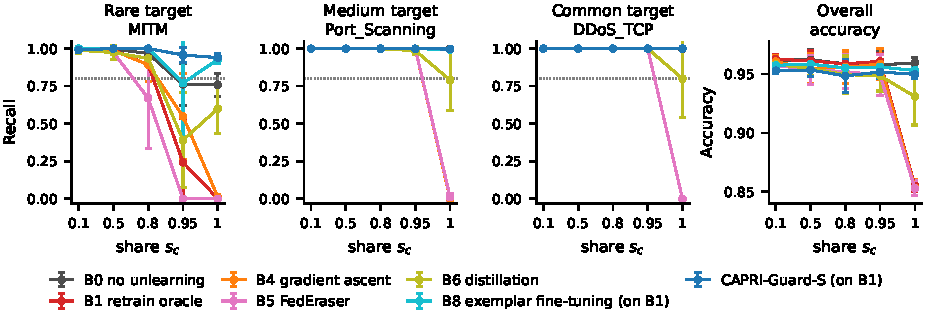
\includegraphics[width=\textwidth]{figures/edge_dose_compact.pdf}
\caption{Dose-response on Edge-IIoTset: target-family recall and overall accuracy against the departing client's share $s_c$ (scenarios S1 to S3; mean and 95\% confidence interval over seeds; dotted line: recall floor $\rho=0.8$). The rare family declines from $s_c=0.8$, the medium and common families are lost only at $s_c=1$, and accuracy does not reveal the rare-family loss. The repair methods keep all three families in every scenario.}\label{fig:dose}
\end{figure*}

The loss is operationally silent. On Edge-IIoTset in S3, the retrain oracle classifies <<pct(v('S3','B1','silent_rare','edge'),0)>> of MITM, <<pct(v('S3','B1','silent_medium','edge'),0)>> of Port\_Scanning and <<pct(v('S3','B1','silent_common','edge'),0)>> of DDoS\_TCP test records as benign (Fig.~\ref{fig:confusion}). Overall accuracy falls by <<f(v('S3','B0','accuracy','edge')-v('S3','B1','accuracy','edge'))>>, close to the targets' <<pct(target_share('edge'),1)>> share of test traffic; when only the rare family is lost (S2c), accuracy changes by <<f(abs(v('S2c','B0','accuracy','edge')-v('S2c','B1','accuracy','edge')))>>. Penultimate-layer embeddings (Appendix~\ref{app:figs}) show that the lost families remain separable in feature space: what is lost is the mapping to the correct output class.

\begin{figure*}[t]
\centering
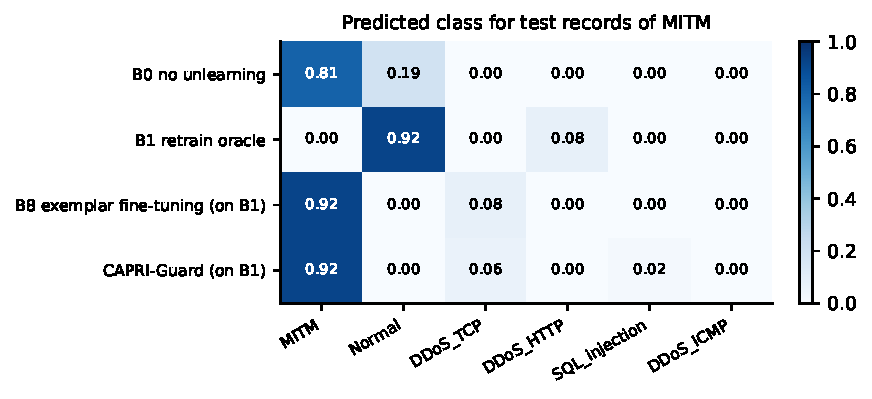
\includegraphics[width=0.92\textwidth]{figures/edge_fig_confusion_rare.pdf}
\caption{Qualitative example (Edge-IIoTset, S3, seed 0): row-normalised predictions for MITM test records before deletion, after the retrain oracle, after exemplar fine-tuning (B8) and after CAPRI-Guard-S. After deletion most MITM records are predicted as Normal traffic (silent misses); after repair they are again predicted as MITM.}\label{fig:confusion}
\end{figure*}

\paragraph{Forgetting.} No model memorises individual records: even the pre-deletion model is as accurate on client 0's records as on unseen records of the same classes (gap <<f(v('S3','B0','forget_gap','edge'),4)>>), and every model's membership-inference AUC lies within <<f(max(max(abs(DS[k]['df'][DS[k]['df'].scenario==sc].groupby('method').mia_auc.mean()-0.5).max() for sc in ['S1','S3']) for k in DS),3)>> of chance on both datasets. Membership inference therefore cannot distinguish forgetting from not forgetting in this setting; what deletion removes is the family, not individual records.

\subsection{RQ2: predicting the loss before deletion}\label{sec:res-rq2}

Table~\ref{tab:audit} evaluates the audit on all family-deletions whose pre-deletion recall was at least $\rho$. On families that other clients still hold ($m_c>0$), where counts carry little information, the audit on Edge-IIoTset finds <<audit('m_c > 0 (non-trivial)','CAPRI-Audit (all signals)','tp','edge')>> of <<audit('m_c > 0 (non-trivial)','CAPRI-Audit (all signals)','n_at_risk','edge')>> at-risk families and outperforms the counts rule (F1 <<f(audit('m_c > 0 (non-trivial)','CAPRI-Audit (all signals)','f1','edge'))>> versus <<f(audit('m_c > 0 (non-trivial)','Rule-only (counts)','f1','edge'))>>, $p=$ <<fp(auditp('perm_test_f1_audit_vs_rule_mc>0','edge')['p_one_sided'])>>). Within CICIoT2023 it does not (<<f(audit('m_c > 0 (non-trivial)','CAPRI-Audit (all signals)','f1','cic'))>> versus <<f(audit('m_c > 0 (non-trivial)','Rule-only (counts)','f1','cic'))>>, $p=$ <<fp(auditp('perm_test_f1_audit_vs_rule_mc>0','cic')['p_one_sided'])>>): there the at-risk cases are shifts between near-identical flood variants, which the departing client's signals describe poorly. Fitted on one dataset and applied to the other, the audit beats the rule in both directions, significantly when fitted on CICIoT2023. On all families the rule is at least as good, because sole-held losses follow from $m_c=0$ alone. The audit is a high-recall, low-precision screen (recall <<f(min(audit('m_c > 0 (non-trivial)','CAPRI-Audit (all signals)','recall',k) for k in DS),2)>>--<<f(max(audit('m_c > 0 (non-trivial)','CAPRI-Audit (all signals)','recall',k) for k in DS),2)>>, precision <<f(min(audit('m_c > 0 (non-trivial)','CAPRI-Audit (all signals)','precision',k) for k in DS),2)>>--<<f(max(audit('m_c > 0 (non-trivial)','CAPRI-Audit (all signals)','precision',k) for k in DS),2)>>), and Laplace noise on the clients' label counts ($\varepsilon=1$, $0.5$) leaves its F1 unchanged (Appendix~\ref{app:tables}).

\begin{table*}[t]
\caption{Pre-deletion audit. Precision (P), recall (R) and F1 of the at-risk flags on families other clients still hold ($m_c>0$) and F1 on all families; $p$: one-sided paired permutation test of audit F1 against the counts rule on $m_c>0$. Arrows denote leave-one-dataset-out fits.}\label{tab:audit}
\scriptsize
\setlength{\tabcolsep}{3pt}
\begin{tabular*}{\textwidth}{@{\extracolsep\fill}lccccccc}
\toprule
 & \multicolumn{5}{c}{$m_c>0$ (non-trivial)} & \multicolumn{2}{c}{All families} \\
\cmidrule(lr){2-6}\cmidrule(lr){7-8}
Fit $\rightarrow$ evaluation & P & R & F1 & Rule F1 & $p$ & F1 & Rule F1 \\
\midrule
<<T_audit()>>
\botrule
\end{tabular*}
\end{table*}

\subsection{RQ3: repairing the lost families}\label{sec:res-rq3}

Table~\ref{tab:basecmp} reports the repair results in S3. On Edge-IIoTset, CAPRI-Guard-S restores the targets after every base method (mean target recall <<f(tgt('S3','Guard[B1]','edge'))>>, <<f(tgt('S3','Guard[B4]','edge'))>> and <<f(tgt('S3','Guard[B5]','edge'))>> after B1, B4 and B5) and lowers the deficit below its pre-deletion value (<<m('S3','B0','dd_deficit',2,'edge')>>), because the exemplars also strengthen families that were weak from the start. Collateral loss rises moderately (<<m('S3','Guard[B1]','col_vs_pre',3,'edge')>> against <<m('S3','B1','col_vs_pre',3,'edge')>> for B1). The MIA safeguard was never triggered (<<guard_reruns()>> of <<guard_runs()>> repairs). Pooled over both datasets and S1--S3, Guard-S has a significantly lower deficit than every unlearning baseline and the lawful oracle (Holm $p\le$ <<fp(max(comb('table_h3_pooled.csv').query("~comparison.str.contains('B8')").p_holm))>>; Appendix Table~\ref{tab:h3}).



\begin{table*}[t]
\caption{Repair under sole ownership and comparison with the re-implemented base methods (R), on identical data, splits, seeds and detector. Recall: mean over the three target families under shared (S1) and sole (S3) ownership; deficit: DD deficit; FAR: benign false-alarm rate; MIA: membership-inference AUC on client 0's records (0.5 = chance); all S3 columns are means over seeds.}\label{tab:basecmp}
\scriptsize
\setlength{\tabcolsep}{1.5pt}
\begin{tabular*}{\textwidth}{@{\extracolsep\fill}lcccccccccc@{}}
\toprule
 & \multicolumn{5}{c}{Edge-IIoTset} & \multicolumn{5}{c}{CICIoT2023} \\
\cmidrule(lr){2-6}\cmidrule(lr){7-11}
Method & S1 recall & S3 recall & Deficit & FAR & MIA & S1 recall & S3 recall & Deficit & FAR & MIA \\
\midrule
<<T_main_cmp()>>
\botrule
\end{tabular*}
\end{table*}

The hypothesis that CAPRI-Guard also beats exemplar fine-tuning (H3) is not supported. B8, which fine-tunes the same base model on the same $\Efit$ with plain cross-entropy, reaches the same restoration (Table~\ref{tab:basecmp}); Guard-S is not lower than B8 on any base (Holm $p=$ <<fp(min(comb('table_h3_pooled.csv').query("comparison.str.contains('B8')").p_holm))>>), and the Friedman ranking places both in one group, significantly better than the unlearning methods (Appendix Fig.~\ref{fig:cd}). On CICIoT2023 the repair has a clear cost: the benign false-alarm rate rises from <<pct(v('S3','B1','benign_far','cic'),1)>> after B1 to <<pct(v('S3','Guard[B1]','benign_far','cic'),1)>> after Guard-S (B8: <<pct(v('S3','B8[B1]','benign_far','cic'),1)>>). The audit flags <<f(mean_flags('cic'),1)>> of <<n_eval('cic')>> families there (Edge-IIoTset: <<f(mean_flags('edge'),1)>> of <<n_eval('edge')>>), most of which cannot reach the floor because their records overlap with another class, so dual ascent keeps raising their weights and the never-flagged benign class absorbs the cost (Section~\ref{sec:ablation}). Forgetting is preserved: membership-inference AUC and the memorisation gap are equivalent to the lawful oracle within $\pm0.02$ for all bases on both datasets (TOST); forget-set accuracy is higher because the restored families are detected again.





\subsection{Extensions}\label{sec:res-ext}

\paragraph{Before/after leakage.} Publishing the unlearned model can reveal which families the departing client held: scoring each family by its recall drop between the models before and after unlearning identifies families with $s_c\ge0.5$ with an AUC of <<f(leak('edge','B1'))>> (Edge-IIoTset) and <<f(leak('cic','B1'))>> (CICIoT2023) for the retrain oracle. After CAPRI-Guard-S the AUC falls to <<f(leak('edge','Guard[B1]'))>> and <<f(leak('cic','Guard[B1]'))>>, because restored families no longer show a drop (Appendix~\ref{app:tables}).

\paragraph{Sequential deletion and partial participation.} When the remaining nine clients continue training for ten rounds after a repair, mean target recall falls from <<f(p3tgt('sequential','Guard[B1]'))>> to <<f(p3tgt('sequential','mid'))>>: the remaining clients do not hold the restored families, so ordinary federated rounds remove them again. A second deletion behaves like the first (retrain <<f(p3tgt('sequential','B1_2'))>>, Guard-S <<f(p3tgt('sequential','Guard[B1_2]'))>>). With five of ten clients sampled per round, the leave-$u$-out estimate subtracts client 0's update only in the rounds it joined, and results match full participation (Guard-S deficit <<f(p3v('partial0.5','Guard[B1]','dd_deficit'),2)>> versus <<f(p3v('default','Guard[B1]','dd_deficit'),2)>>).

%% ============================================================== 6
\section{Comparison with base papers and state of the art}\label{sec:base}

\paragraph{Base methods.} The base methods are three federated unlearning methods re-implemented and run in the same setting (FedEraser~\cite{liu2021federaser}, gradient ascent~\cite{halimi2022}, distillation~\cite{wu2022distill}), the two federated unlearning methods for intrusion detection, whose results are taken from their publications (ARFU-IDS~\cite{yang2026arfu}, FU-IDS~\cite{wang2026fuids}), and restricted softmax~\cite{li2021fedrs}, on which the training builds (Table~\ref{tab:basesum}).

\begin{table*}[t]
\caption{Summary of the base methods. R: re-implemented and run in this study; *: result as reported in the original publication; FU: federated unlearning.}\label{tab:basesum}
\scriptsize
\setlength{\tabcolsep}{3pt}
\begin{tabular*}{\textwidth}{@{\extracolsep\fill}>{\raggedright\arraybackslash}p{2.2cm}>{\raggedright\arraybackslash}p{1.9cm}>{\raggedright\arraybackslash}p{2.5cm}>{\raggedright\arraybackslash}p{2.6cm}>{\raggedright\arraybackslash}p{2.8cm}>{\raggedright\arraybackslash}p{2.8cm}@{}}
\toprule
Authors (year), method & Problem & Method & Data; metrics & Reported result & Limitation in this setting \\
\midrule
Liu et al.\ (2021), FedEraser~\cite{liu2021federaser}$^{\mathrm{R}}$ & Client removal in FL & Calibrated stored client updates & Adult, Purchase, MNIST, CIFAR-10; accuracy, speed-up & Expected $4\times$ speed-up over retraining* & Reproduces retraining, including the sole-held loss \\
Halimi et al.\ (2022)~\cite{halimi2022}$^{\mathrm{R}}$ & Client removal in FL & Projected gradient ascent, then few FL rounds & MNIST, EMNIST, CIFAR-10; backdoor accuracy, MIA & Comparable to retraining at lower cost* & Same retraining criterion; needs the client \\
Wu et al.\ (2022)~\cite{wu2022distill}$^{\mathrm{R}}$ & Right to be forgotten in FL & Update subtraction, distillation restore & MNIST, CIFAR-10, GTSRB; accuracy, backdoor & Effective without client data* & Distillation retains forgotten knowledge \\
Yang et al.\ (2026), ARFU-IDS~\cite{yang2026arfu} & FU for IDS, keep rare attacks & Attention-head attribution, verification & UNSW-NB15, CICIoT2023, IoTID20; macro-F1, rare recall & 87.1\% macro-F1, 77.6\% pooled rare recall, within 0.2\,pp of retraining* & Retraining as success; pooled recall; transformer-specific \\
Wang et al.\ (2026), FU-IDS~\cite{wang2026fuids} & FU for anomaly detection & Neuron-level gradient scaling, audit & UNSW-NB15, CICIoT2023, IoTID20; rare recall, false-positive rate & 73.9\% pooled rare recall, 2.4\% false-positive rate, $35\times$ faster than retraining* & Audits memorisation, not lost capability \\
Li and Zhan (2021), FedRS~\cite{li2021fedrs} & FL under label skew & Restricted softmax for missing classes & Public data, one application; accuracy & Improves FedAvg under label skew* & Training method, used here with $\alpha_{\mathrm{RS}}=0$ \\
\botrule
\end{tabular*}
\end{table*}

\paragraph{Quantitative comparison.} Table~\ref{tab:basecmp} (Section~\ref{sec:res-rq3}) compares CAPRI with the re-implemented base methods on identical data, splits, seeds, detector and metrics. Under shared ownership, the setting in which these methods are normally evaluated, all of them keep the target families, consistent with their published claims. Under sole ownership, FedEraser and gradient ascent lose the targets as completely as the retrain oracle they approximate, and distillation keeps part of them only because it forgets less. Adding CAPRI-Guard-S restores the targets with membership inference at chance level.



ARFU-IDS and FU-IDS were evaluated on UNSW-NB15 with transformer detectors and their code is not publicly available, so their figures (Table~\ref{tab:basesum}, marked *) are not directly comparable. The comparable quantity is the success criterion. ARFU-IDS reports staying within 0.2 percentage points of retraining*; under shared ownership the re-implemented methods here are likewise within <<f(100*max(abs(tgt('S1',mm,'edge')-tgt('S1','B1','edge')) for mm in ['B4','B5']),1)>> points, but under sole ownership the retraining reference itself has target recall <<f(tgt('S3','B1','edge'))>>. A pooled rare-category recall (77.6\%*, 73.9\%*) hides the same effect: in S3 the mean recall over the <<n_eval('edge')>> evaluable Edge-IIoTset families falls only from <<f(csv('table_per_family_recall.csv','edge',header=[0,1],index_col=0)[('S3','B0')].mean())>> to <<f(csv('table_per_family_recall.csv','edge',header=[0,1],index_col=0)[('S3','B1')].mean())>> while three families are lost completely.

\paragraph{Methodological comparison.} The base methods differ in how they approximate the retrain oracle; CAPRI changes what is optimised. First, it adds a pre-deletion step that the base methods lack: the audit warns which families a deletion will cost, using the stored history that FedEraser and Wu et al.\ already require. Second, the repair objective (Eq.~\ref{eq:guard}) contains an explicit per-family recall floor rather than closeness to retraining, which addresses the limitation that all base methods share. Third, the repair draws only on data held independently of the departing client, and forgetting is judged against the lawful oracle, so restored capability is not confused with residual knowledge, unlike distillation from the original model~\cite{wu2022distill}, which retains part of the forgotten client's knowledge (Table~\ref{tab:rq1}).

\paragraph{Improvement analysis.} Table~\ref{tab:improve} gives the absolute and relative change achieved by adding CAPRI-Guard-S. On Edge-IIoTset it raises the target recall by about 97 percentage points over FedEraser and gradient ascent and reduces the deficit by roughly three quarters, at a cost of less than one percentage point of benign false alarms. On CICIoT2023 the deficit falls by <<f(-rel(v('S3','Guard[B5]','dd_deficit','cic'),v('S3','B5','dd_deficit','cic')),0)>>--<<f(-rel(v('S3','Guard[B4]','dd_deficit','cic'),v('S3','B4','dd_deficit','cic')),0)>>\% only, because about <<f(v('S1','B0','dd','cic'),0)>> of its <<n_eval('cic')>> families are below the floor even before deletion, and the false-alarm cost is large. The gain comes from the lawful exemplars: the same comparison against exemplar fine-tuning (last row) shows no improvement in recall or deficit.

\begin{table*}[t]
\caption{Improvement of CAPRI-Guard-S over each base method in S3: change in mean target recall (percentage points), in DD deficit (absolute and relative) and in benign false-alarm rate (percentage points). Guard-S is applied after FedEraser and gradient ascent; for distillation and B8 it is applied after the retrain oracle.}\label{tab:improve}
\scriptsize
\setlength{\tabcolsep}{2.5pt}
\begin{tabular*}{\textwidth}{@{\extracolsep\fill}lcccccc}
\toprule
 & \multicolumn{3}{c}{Edge-IIoTset} & \multicolumn{3}{c}{CICIoT2023} \\
\cmidrule(lr){2-4}\cmidrule(lr){5-7}
Over & Recall & Deficit & FAR & Recall & Deficit & FAR \\
\midrule
<<T_improve()>>
\botrule
\end{tabular*}
\end{table*}

\paragraph{Fairness of the comparison.} The re-implemented methods follow their publications but were adapted to tabular data and an MLP (B4 with a fixed ascent budget, B6 distilling on unlabelled exemplar features); all methods share the same pre-deletion model. The ARFU-IDS and FU-IDS figures come from a different dataset, detector, partition and pooled metrics and are shown for context only. Because duplicates are removed after dropping identifiers (<<pct(1-total('edge')/raw_edge(),1)>> of Edge-IIoTset), accuracy figures are not comparable with studies that keep them~\cite{bilal2026,peng2025fdids}. CAPRI does not outperform exemplar fine-tuning, and on CICIoT2023 it is worse in benign false alarms (Section~\ref{sec:ablation}).

%% ============================================================== 7
\section{Ablation study}\label{sec:ablation}

Each component of CAPRI-Guard-S was removed or replaced in S3, on all ten seeds and all three base methods (Table~\ref{tab:ablation}; mean\,$\pm$\,s.d.\ for base B1 in Appendix Fig.~\ref{fig:ablation}).

\begin{table*}[t]
\caption{Ablation of CAPRI-Guard-S in S3 (mean over 3 bases\,$\times$\,10 seeds). $^{\dagger}$: different from full Guard-S (two-sided paired Wilcoxon, Holm-corrected, $p<0.05$).}\label{tab:ablation}
\scriptsize
\setlength{\tabcolsep}{3pt}
\begin{tabular*}{\textwidth}{@{\extracolsep\fill}lcccccc}
\toprule
 & \multicolumn{3}{c}{Edge-IIoTset} & \multicolumn{3}{c}{CICIoT2023} \\
\cmidrule(lr){2-4}\cmidrule(lr){5-7}
Variant & DD deficit & Collateral loss & FAR & DD deficit & Collateral loss & FAR \\
\midrule
<<T_ablation()>>
\botrule
\end{tabular*}
\end{table*}

\begin{itemize}
\item \emph{KL anchor.} The only component with a consistent effect. Without it, collateral loss rises from <<f(abt('Abl-noanchor','col_vs_pre','guard_mean','edge'))>> to <<f(abt('Abl-noanchor','col_vs_pre','variant_mean','edge'))>> and the deficit almost doubles on Edge-IIoTset, and on CICIoT2023 every benign record is flagged as an attack.
\item \emph{Dual ascent.} A fixed weight gives the same deficit on Edge-IIoTset with lower collateral loss, and on CICIoT2023 a lower deficit and far fewer false alarms (<<pct(abt('Abl-fixed','benign_far','variant_mean','cic'),1)>> versus <<pct(abt('Abl-fixed','benign_far','guard_mean','cic'),1)>>). Raising the weights of families that cannot reach the floor pushes the model against its other classes without a net gain.
\item \emph{Proximity term.} No measurable effect, consistent with the absence of record-level memorisation.
\item \emph{Audit targeting.} Flagging every family gives the same deficit on Edge-IIoTset and fewer false alarms on CICIoT2023; targeting does not reduce side-effects as expected. Flags from the counts rule cover only the sole-held families, so the remaining weak families stay unrepaired and the deficit is about twice as large on Edge-IIoTset.
\end{itemize}



\paragraph{Sensitivity.} The deficit falls steeply with the number of exemplars (with 4 per class the rare target already recovers to <<m('S3','Sweep-k4[B1]','recall_rare',2,'edge')>>), worsens for a recall floor of 0.5, and degrades gradually with 10--20\% exemplar label noise, which however raises false alarms to <<pct(v('S3','Sweep-noise0.2[B1]','benign_far','edge'),1)>> (Appendix Fig.~\ref{fig:sens}). The loss and its repair persist under stronger and weaker label skew, 20 clients, a one-dimensional convolutional network (1D-CNN), unweighted training and partial participation, with Guard-S and B8 always within <<f(max(abs(p3t(x,'Guard[B1] vs B8[B1]','mean_diff')) for x in ['alpha0.1','alpha1.0','K20','cnn','unweighted','partial0.5']),2)>> deficit units of each other (Appendix Table~\ref{tab:pass3}); membership-inference AUC stays at chance throughout.



%% ============================================================== 8
\section{Discussion}\label{sec:discussion}

\paragraph{Why the loss occurs and why repair works.} A sole-held family is lost because no remaining client supplies evidence for its output class, so the retrain oracle, and every method that approximates it, assigns its records to the most similar remaining class, usually benign traffic. The families stay separable in feature space, so a little labelled data restores the mapping: 25 fitting exemplars per class and plain fine-tuning suffice. The anchor to the unlearned model limits side-effects; the constrained mechanism adds nothing measurable beyond that.

\paragraph{Practical implications.} Per-family evaluation is necessary, because matching retraining, pooled rare recall and overall accuracy all hide the loss. A pre-deletion audit from data the server already stores is a high-recall screen that should trigger review, not automatic action. An operator that must honour a deletion and keep detecting the departing member's families needs independently held exemplars, a repair that protects the benign class, and protection of restored families during later training.

\paragraph{Strengths.} A fully paired design with ten seeds for the headline comparison, two datasets, pre-specified hypotheses, multiple-comparison correction and effect sizes; strict leakage control; a fair control for the repair (B8), which exposes the main negative result; and every number regenerated from logged outputs.

\paragraph{Limitations and failure cases.} The audit's advantage did not hold within CICIoT2023, and CAPRI-Guard did not outperform exemplar fine-tuning; on CICIoT2023 it raised benign false alarms to <<pct(v('S3','Guard[B1]','benign_far','cic'),0)>> and lowered target recall under shared ownership from <<f(tgt('S1','B1','cic'))>> to <<f(tgt('S1','Guard[B1]','cic'))>>. A sole-held family is not always learned before deletion (CICIoT2023 common target below $\rho$ in <<int((sel('S3','B0','cic').recall_common<RHO).sum())>> of <<nseeds('S3','cic')>> S3 seeds), and repairs decay under continued training.

\paragraph{Threats to validity.} \emph{Internal:} the base methods were re-implemented for tabular data, and restricted softmax was needed for sole-held families to be learned; results with plain FedAvg would differ. \emph{Construct:} loss-threshold membership inference is at chance for every model after deduplication, so the forgetting evidence rests on forget-set accuracy, relearning and the memorisation gap; shadow-model attacks~\cite{shokri2017} and backdoor-based verification were not run. \emph{External:} two IoT datasets, one departing client per deletion and one detector family in the main design. A column shift in the DNS query-name length field of <<num(DNS['non_numeric'])>> Edge-IIoTset records (<<pct(DNS['share'],2)>>, all Normal) affects only benign traffic. \emph{Conclusion:} five-seed sensitivity analyses are descriptive.

\paragraph{Were the research gap and objectives met?} The gap that no evaluation removes the sole holder of an attack family and reports per-family detection is addressed: RQ1 is answered with strong evidence on both datasets. RQ2 is answered partly: the loss is predictable from server-side information, but the learned audit's advantage over a simple rule is not stable. RQ3 is answered with a qualification: capability can be restored without weakening forgetting, but the restoration comes from lawful exemplars rather than from CAPRI-Guard's specific mechanism.

%% ============================================================== 9
\section{Conclusion and future work}\label{sec:conclusion}

Federated unlearning, including exact retraining, removes the detection of an attack family whose sole holder departs; the lost attacks are mostly classified as benign, and neither accuracy nor closeness to retraining reveals the loss. A pre-deletion audit from the stored update history finds most at-risk families with low precision, and a small lawful exemplar set restores the lost families without measurable memorisation, with plain fine-tuning as effective as the proposed repair. Future work should protect restored families during continued training, add a benign-class constraint to the repair, improve the audit's precision for near-identical attack variants, and extend the evaluation to further datasets, detectors and multiple or adversarial deletion requests.

%% ============================================================== declarations
\backmatter

\bmhead{Acknowledgements}
The authors thank the providers of the Edge-IIoTset and CICIoT2023 datasets.

\section*{Declarations}\label{sec:decl}

\begin{itemize}
\item \textbf{Funding:} No funding was received for this study.
\item \textbf{Competing interests:} The authors declare no competing interests.
\item \textbf{Ethics approval and consent to participate:} Not applicable; only public datasets are used and no human participants are involved.
\item \textbf{Consent for publication:} Not applicable.
\item \textbf{Data availability:} Edge-IIoTset~\cite{ferrag2022} and CICIoT2023~\cite{neto2023} are publicly available from their authors; file hashes, the sampling procedure and all seeds are provided with the code.
\item \textbf{Materials availability:} Not applicable.
\item \textbf{Code availability:} Implementation, logged outputs of all <<len(DS['edge']['p1'])+len(DS['cic']['p1'])+35>> runs and the scripts that regenerate every table and figure: <<CODE_URL>>.
\item \textbf{Author contribution:} Ibrahim Ghauri and Okasha Yamin contributed equally to this work; both authors read and approved the final manuscript.
\item \textbf{AI-tool usage:} An AI assistant (a large language model) was used in this study to assist with the literature analysis, writing and debugging the implementation and analysis code, running the experiments, and drafting and editing the text of this paper. The authors directed the work, reviewed all code, text and results, approved the final version of the paper and take full responsibility for its content. Every reported number is computed by the released code from the logged experiment outputs.
\end{itemize}

\bibliography{references}

\clearpage
\onecolumn
\begin{appendices}

\FloatBarrier
\section{Changes from the original methodology}\label{app:changes}

\begin{table}[!htbp]
\caption{Changes from the original methodology and their reasons.}\label{tab:changes}
\footnotesize
\begin{tabular*}{\textwidth}{@{\extracolsep\fill}>{\raggedright\arraybackslash}p{4.6cm}>{\raggedright\arraybackslash}p{10.8cm}@{}}
\toprule
Change & Reason \\
\midrule
Restricted softmax ($\alpha_{\mathrm{RS}}=0$) in local training & With plain FedAvg the sole-held targets were never learned before deletion (pilot: recall 0.00); $\alpha=0.5$ did not resolve this. \\
Early stopping patience 5$\rightarrow$10, minimum 20 rounds & Validation macro-F1 fluctuates; with patience 5 the pilot stopped at round 7. \\
Learnability gate for target families & A family a centralised reference model cannot learn (validation recall $<0.8$) cannot lose capability; the gate is decided on validation data before any deletion result. \\
Duplicate grouping across splits & No feature vector is shared between exemplar, test, validation and client data, which is stricter than removing test duplicates. \\
Audit fitted leave-one-seed-out; leave-one-dataset-out reported separately & Flags used by the repair never see their own deletion's outcome. \\
CICIoT2023 cap applied to unique records & Later deduplication cannot push a capped class below the cap. \\
Cross-dataset exemplar test not run & The two releases share almost no feature definitions (per-packet fields versus window statistics). \\
B6 distillation set & Unlabelled exemplar features, the same data CAPRI-Guard holds. \\
Federated simulation in PyTorch instead of a federated framework & Vectorised training of all clients and storage of every round's updates, which the audit and FedEraser require. \\
Exemplar sweep $q\in\{0,4,10,20,50\}$ & The pool holds 50 records per class. \\
$\gamma=10^{-2}$ default (planned $10^{-3}$); sweep $\{10^{-3},10^{-2},10^{-1}\}$ & The implemented default differed from the plan; the planned value is in the sweep and gives the same results; $\gamma=0$ is covered by the ablation. \\
Page's trend test instead of a binomial GLM for dose-response & Recall is a step function of $s_c$ for medium and common families, so the GLM has no finite maximum. \\
Added: forget-set minus class-matched test accuracy & Membership inference is at chance for every model; this measure separates record memorisation from family capability. \\
Not run: shadow-model MIA, backdoor verification runs, B7 & Not implemented in this phase (MIA, backdoor); B7 code is not publicly available. \\
\botrule
\end{tabular*}
\end{table}

Table~\ref{tab:changes} lists every deviation from the original methodology and its reason.

\FloatBarrier
\section{Additional results}\label{app:tables}

\begin{table}[!htbp]
\caption{Design sensitivity on Edge-IIoTset (S3, 5 seeds): target recall before deletion (B0) and after the retrain oracle (B1), DD deficit of B1, B8 and Guard-S, and two-sided Wilcoxon $p$ of Guard-S versus B8.}\label{tab:pass3}
\scriptsize
\setlength{\tabcolsep}{2pt}
\begin{tabular*}{\textwidth}{@{\extracolsep\fill}lcccccc}
\toprule
Setting & B0 & B1 & \multicolumn{3}{c}{Deficit B1 / B8 / Guard} & $p$ \\
\midrule
<<T_pass3()>>
\botrule
\end{tabular*}
\end{table}

\begin{table}[!htbp]
\caption{Before/after leakage: ROC AUC of the recall drop for identifying families with $s_c\ge0.5$ (S2a--S3; 0.5 = no information).}\label{tab:leak}
\footnotesize
\begin{tabular*}{\textwidth}{@{\extracolsep\fill}lcc}
\toprule
Method & Edge-IIoTset & CICIoT2023 \\
\midrule
<<T_ext()>>
\botrule
\end{tabular*}
\end{table}

Table~\ref{tab:hyper} lists the hyperparameters, Table~\ref{tab:h3} the H3 tests, Table~\ref{tab:pass3} the design sensitivity and Table~\ref{tab:leak} the before/after leakage test. With Laplace noise on the clients' label counts, the audit's F1 on $m_c>0$ is <<f(priv('edge','1.0','CAPRI-Audit','f1_mean'))>> ($\varepsilon=1$) and <<f(priv('edge','0.5','CAPRI-Audit','f1_mean'))>> ($\varepsilon=0.5$) on Edge-IIoTset against <<f(priv('edge','none','CAPRI-Audit','f1_mean'))>> without noise, and <<f(priv('cic','1.0','CAPRI-Audit','f1_mean'))>> and <<f(priv('cic','0.5','CAPRI-Audit','f1_mean'))>> against <<f(priv('cic','none','CAPRI-Audit','f1_mean'))>> on CICIoT2023 (20 draws).

\begin{table}[!htbp]
\caption{Hyperparameters (fixed before the main runs).}\label{tab:hyper}
\scriptsize
\begin{tabular*}{\textwidth}{@{}p{1.9cm}p{5.4cm}@{}}
\toprule
Component & Setting \\
\midrule
FedAvg & 10 clients, $\le$50 rounds, 2 local epochs, batch 256, Adam $10^{-3}$ \\
Early stopping & validation macro-F1, patience 10, min.\ 20 rounds \\
Restricted softmax & $\alpha_{\mathrm{RS}}=0$~\cite{li2021fedrs} \\
Exemplars & $q=50$ per class (25 in $\Efit$, 25 in $\Echk$) \\
CAPRI-Guard & $\rho=0.8$, $\gamma=10^{-2}$, $\eta=1$, $\lambda_{\max}=10$, $\lambda_c$ initialised to 1, $E_{\mathrm{G}}=20$ epochs, Adam $10^{-3}$, batch 64 \\
Guard-F & 3 federated rounds interleaved with repair \\
B3 / B4 & 5 rounds / 1 ascent epoch (lr 0.01) + 5 rounds \\
B5 & calibration every 2nd round, 1 local epoch \\
B6 & 20 epochs, temperature 2, Adam $10^{-3}$, batch 64 \\
Relearning budget & 300 fine-tuning steps \\
Seeds & 0--9 (S1, S3), 0--4 (S0, S2a--c) \\
\botrule
\end{tabular*}
\end{table}

\begin{table}[!htbp]
\caption{H3 tests on the detection-debt deficit (Guard-S minus comparison; negative favours Guard-S): mean difference per dataset and pooled over S1--S3; one-sided Wilcoxon, Holm-corrected (pooled).}\label{tab:h3}
\scriptsize
\begin{tabular*}{\textwidth}{@{\extracolsep\fill}lccccc}
\toprule
Comparison & Edge & CIC & Pooled & $r_{\mathrm{rb}}$ & $p$ \\
\midrule
<<T_h3()>>
\botrule
\end{tabular*}
\end{table}

\clearpage
\section{Additional figures}\label{app:figs}

\begin{figure}[!htbp]
\centering
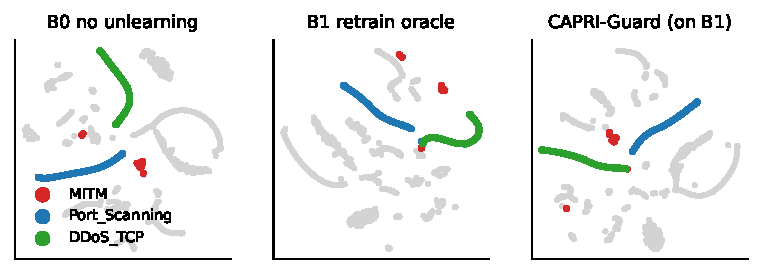
\includegraphics[width=0.81\textwidth]{figures/edge_fig_embeddings.pdf}
\caption{t-SNE~\cite{vandermaaten2008} of penultimate-layer embeddings (Edge-IIoTset, S3, seed 0) before deletion, after the retrain oracle and after CAPRI-Guard-S, with the three target families highlighted. The families remain separable after unlearning (qualitative view, not used for any test).}\label{fig:emb}
\end{figure}

\begin{figure}[!htbp]
\centering
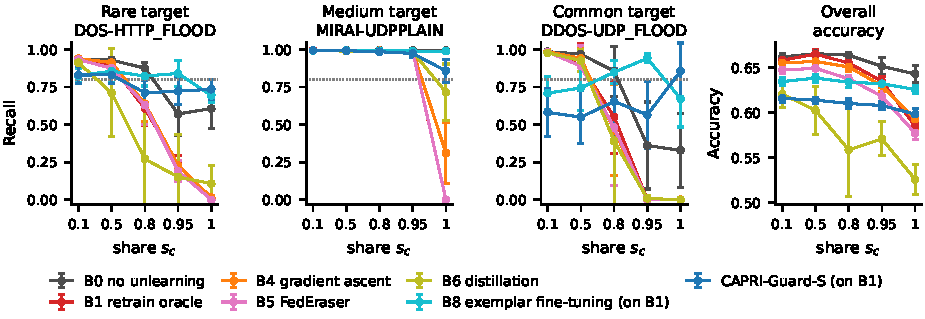
\includegraphics[width=\textwidth]{figures/cic_dose_compact.pdf}
\caption{Dose-response on CICIoT2023 (as Fig.~\ref{fig:dose}). The rare and common targets decline from $s_c=0.8$; the medium target only at $s_c=1$.}\label{fig:dose-cic}
\end{figure}

\begin{figure}[!htbp]
\centering
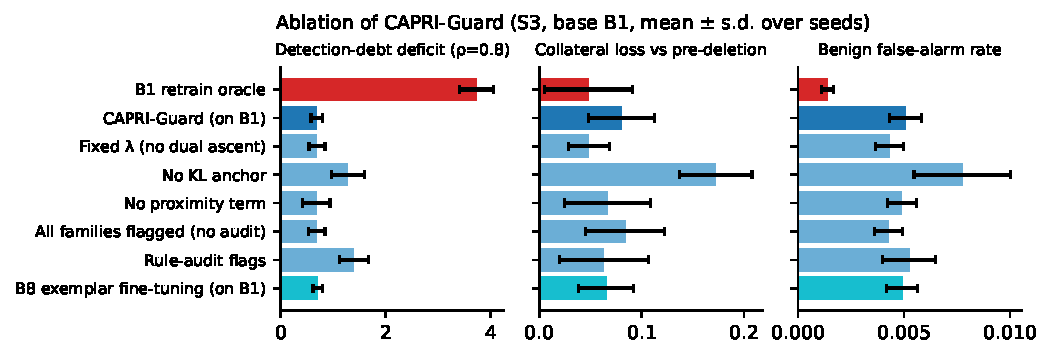
\includegraphics[width=\textwidth]{figures/edge_fig_ablation.pdf}
\caption{Ablation of CAPRI-Guard-S on Edge-IIoTset (S3, base B1): detection-debt deficit, collateral loss and benign false-alarm rate for each variant (mean\,$\pm$\,s.d.\ over seeds).}\label{fig:ablation}
\end{figure}

Fig.~\ref{fig:cd} shows the critical-difference diagram, Fig.~\ref{fig:sens} the sensitivity analysis, Fig.~\ref{fig:emb} the embeddings discussed in Section~\ref{sec:res-rq1}, Fig.~\ref{fig:ablation} the ablation for base B1 and Fig.~\ref{fig:dose-cic} the dose-response on CICIoT2023.

\begin{figure}[!htbp]
\centering
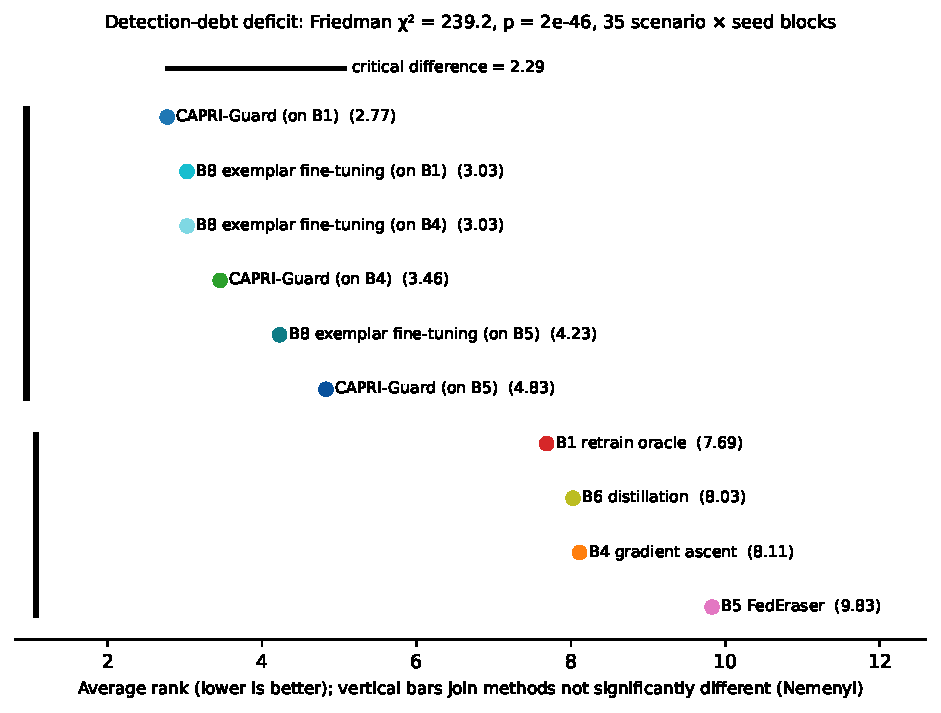
\includegraphics[width=0.85\textwidth]{figures/edge_fig_cd.pdf}
\caption{Critical-difference diagram of the detection-debt deficit on Edge-IIoTset (Friedman test over <<fr('edge')['n_blocks']>> scenario\,$\times$\,seed blocks, $\chi^2=$ <<f(fr('edge')['chi2'],1)>>, $p=$ <<fp(fr('edge')['p'])>>; Nemenyi CD $=$ <<f(fr('edge')['cd'],2)>>). Bars join methods that are not significantly different.}\label{fig:cd}
\end{figure}

\begin{figure}[!htbp]
\centering
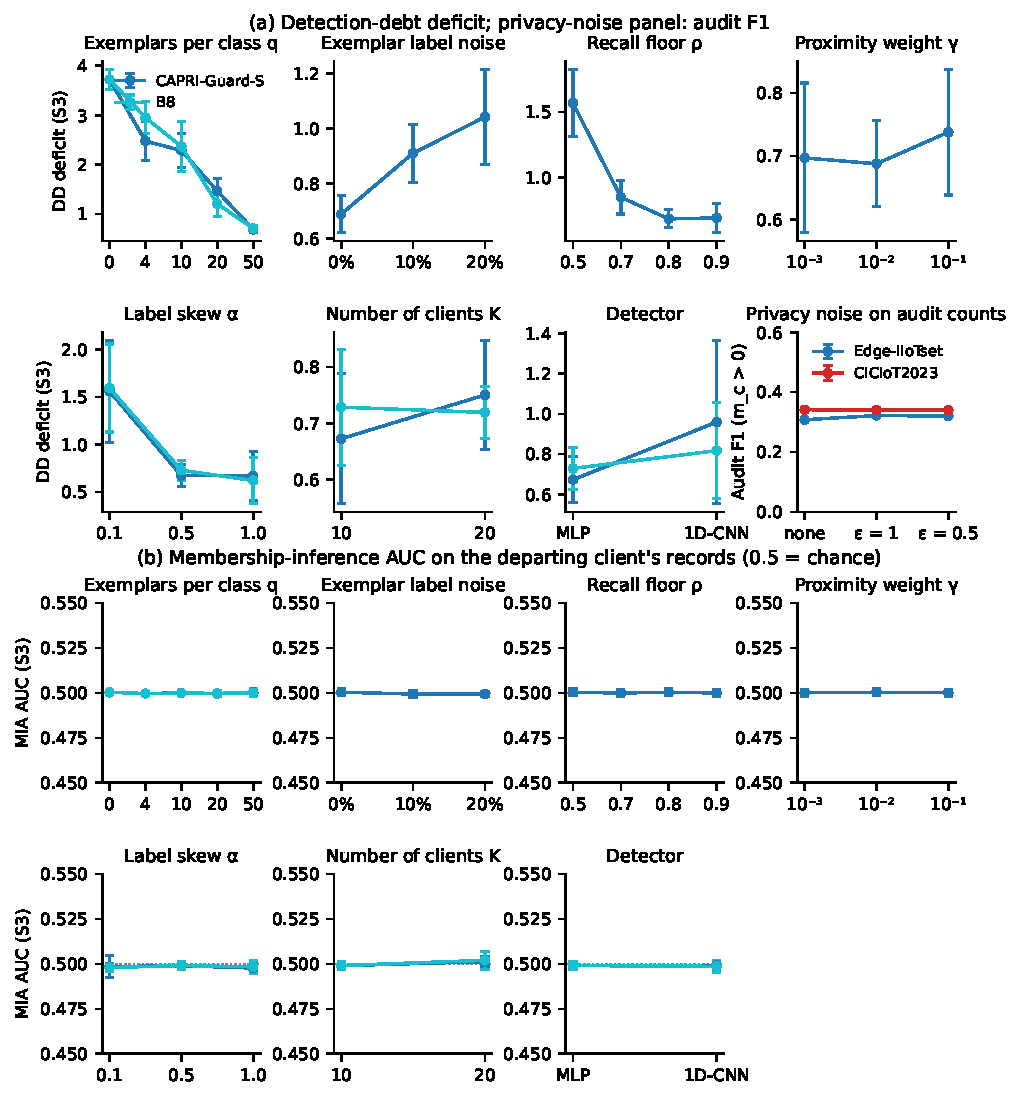
\includegraphics[width=\textwidth]{figures/fig_sensitivity.pdf}
\caption{Sensitivity on Edge-IIoTset (S3, base B1): (a) detection-debt deficit (privacy-noise panel: audit F1 on $m_c>0$ for both datasets) and (b) membership-inference AUC against each factor, for CAPRI-Guard-S and exemplar fine-tuning (B8). Mean and 95\% confidence interval over seeds (10 for exemplar budget, label noise, recall floor and proximity weight; 5 for label skew, number of clients and detector).}\label{fig:sens}
\end{figure}

\FloatBarrier
\end{appendices}


\end{document}
